\chapter{Modell 1: YOLOX}\label{chap:yolox}
\section{Architektur}

\begin{figure}[h]
	\centering
	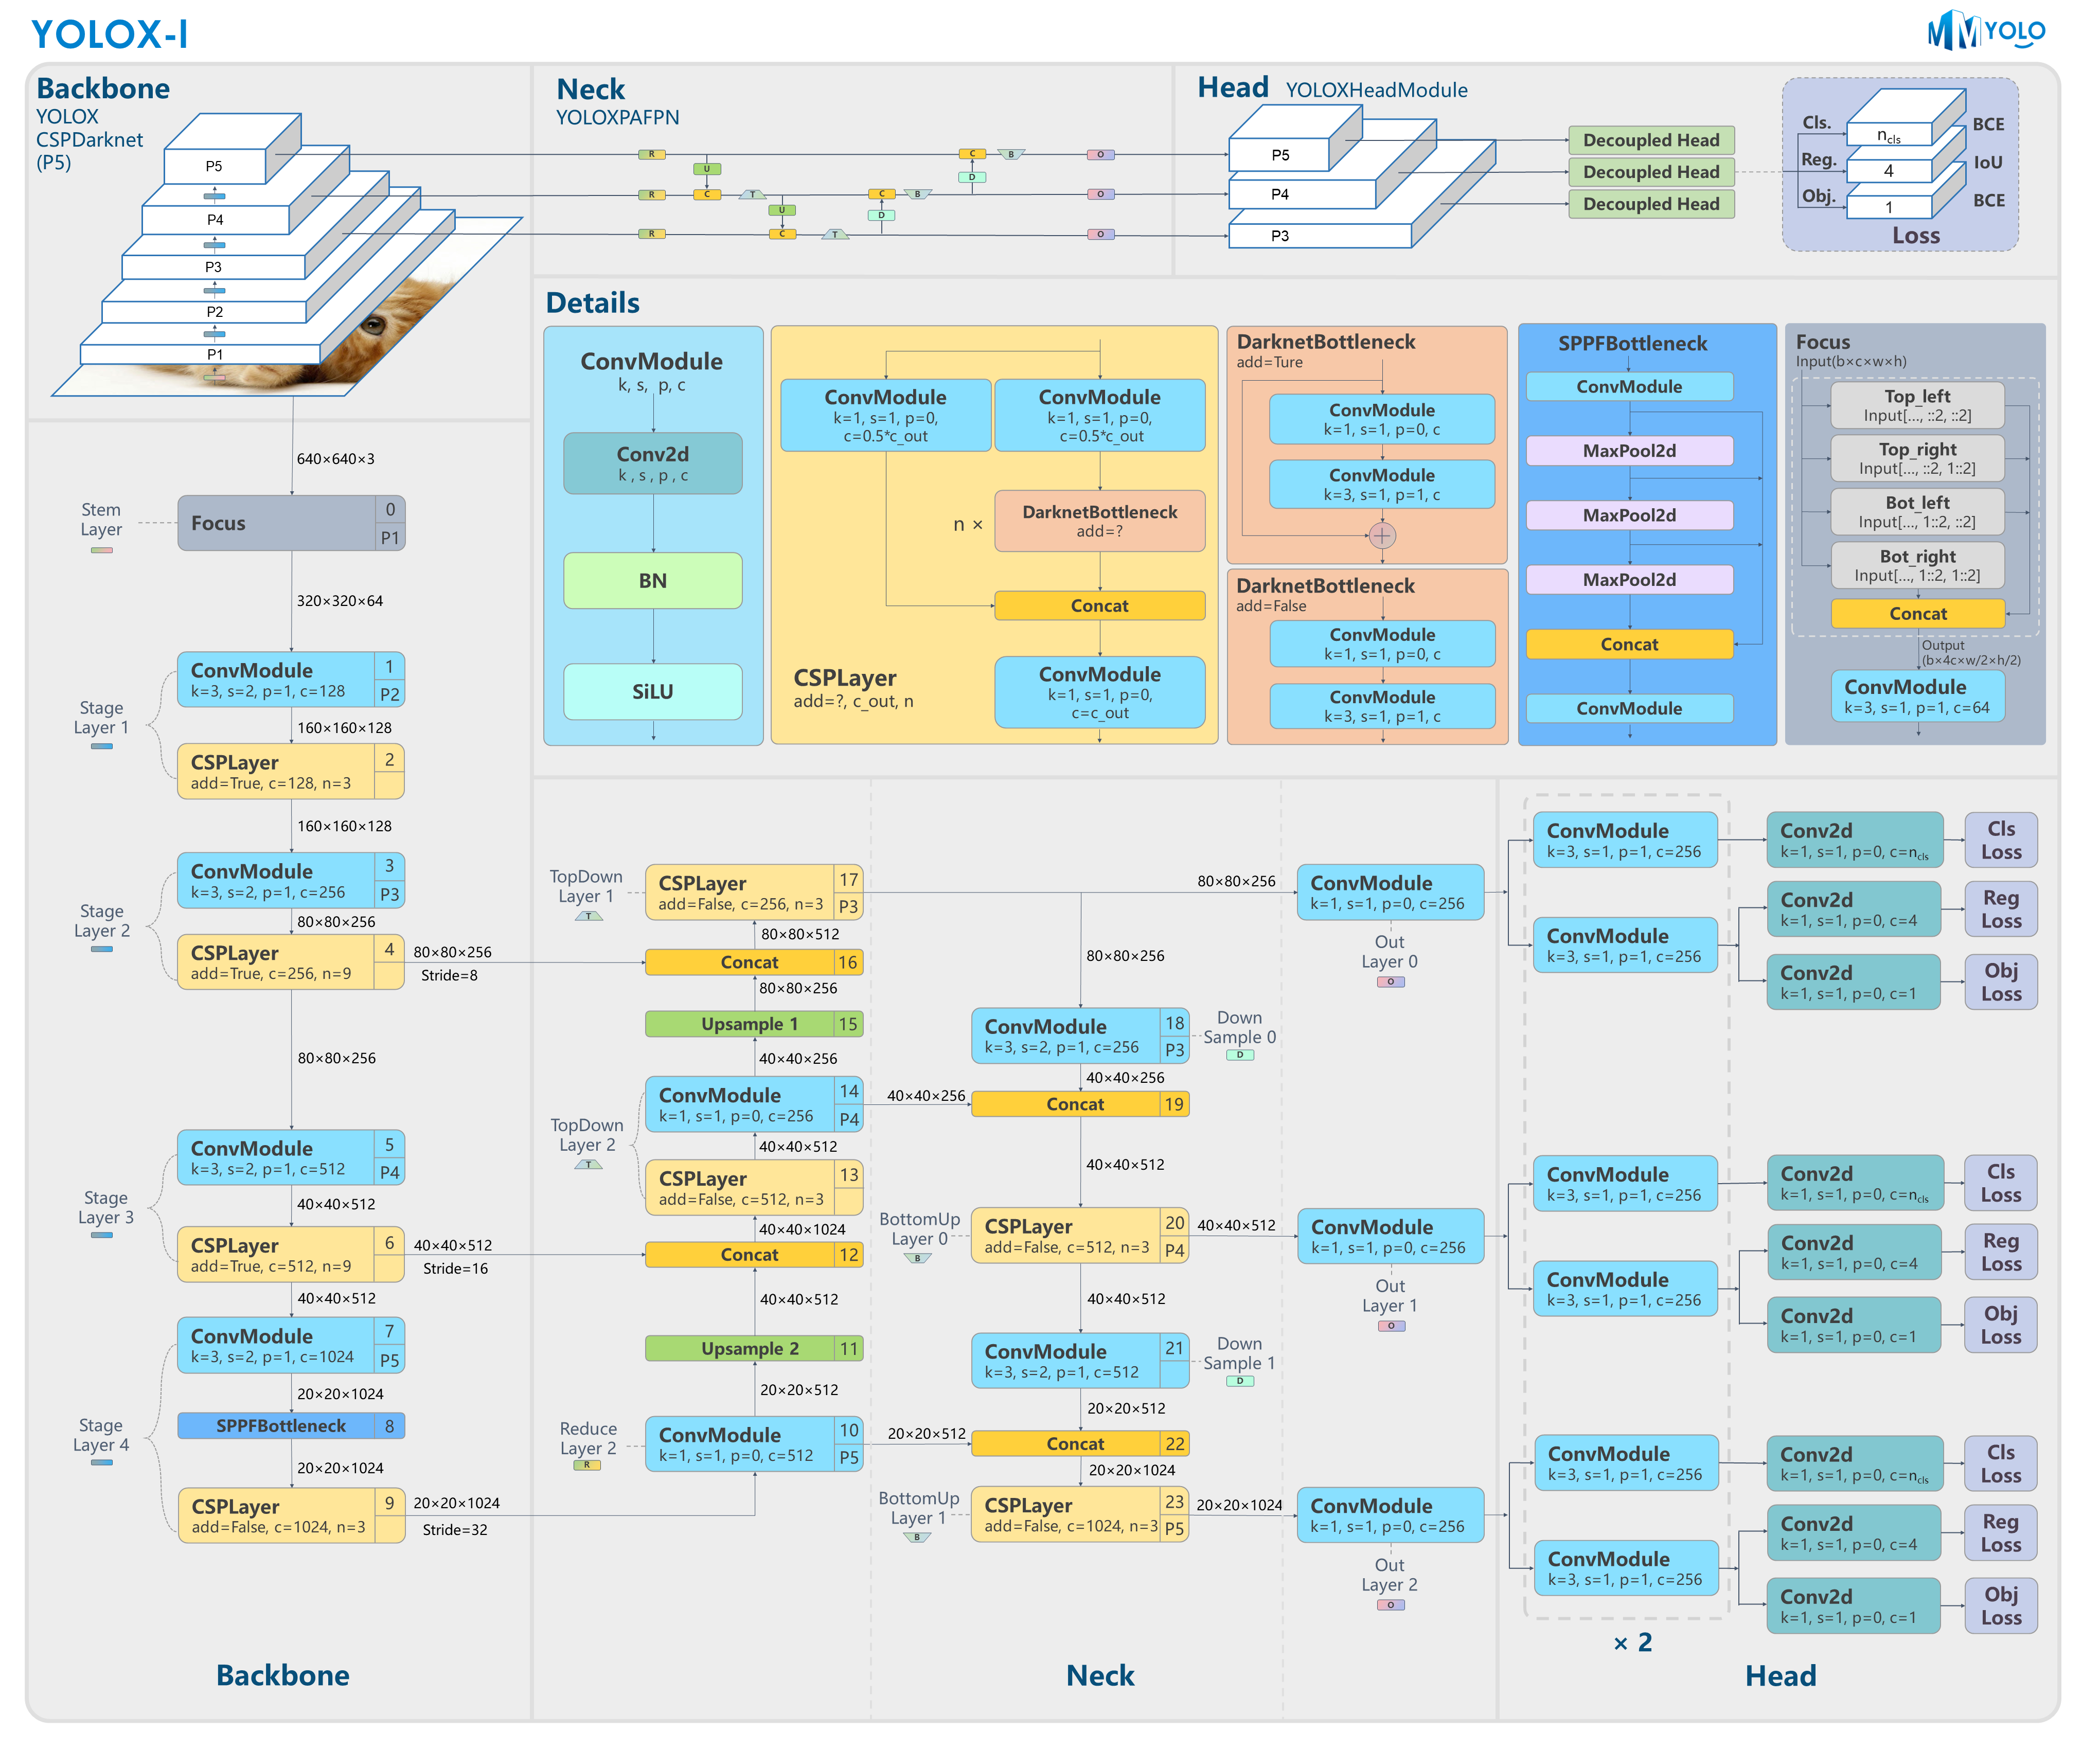
\includegraphics[width=0.8\linewidth]{yoloxArchitecture.png}
	\caption[Übersicht über die Architektur von YOLOX]{Übersicht über die Architektur von YOLOX. Quelle: \cite{yoloArchitecture, yoloxPaper, yoloxGitHubRepo}}
	\label{fig:yoloxArchitecture.png}
\end{figure}

Die YOLOX Architektur besteht aus einem Backbone-Netz, dem Neck und einem Head.

\subsection{Backbone}
YOLOX verwendet das CSPDarknet als Backbone, um Merkmale auf drei verschiedenen Maßstäben zu extrahieren. Die Ausgänge haben Dimensionen von ($H/8$x$W/8$x$256$), ($H/16$x$W/16$x$512$) und ($H/32$x$W/32$x$1024$). Diese Skalierungen ermöglichen die Erzeugung von Merkmalen für unterschiedliche Größen von Objekten. Durch die erhöhte Anzahl von Kanälen wird der Informationsverlust in den kleineren Feature-Maps ausgeglichen. Die tiefere Feature-Map (auf der Abbildung \ref{fig:yoloxArchitecture.png} unten) besitzt ein größeres Receptive Field und ein Pixel kodiert Informationen über einen größeren Bereich des ursprünglichen Bildes.

Das CSPDarknet (Cross Stage Partial) ist eine Modifizierung des ursprünglichen Darknet-Frameworks, das in YOLOv3 schon implementiert wurde. Die Anpassungen bieten Verbesserungen in Bezug auf Geschwindigkeit und Genauigkeit bei der Erkennung von Objekten in Bildern.

CSP steht für Cross Stage Partial Network. Diese Architektur besteht aus einem CSP-Block, der in verschiedenen Stufen des Netzwerks eingefügt ist. Der CSP-Block spaltet den Eingang in zwei Zweige auf, wobei ein Teil unverändert durch den Block läuft und der andere Teil durch eine Kombination aus Faltungsoperationen und Verbindungsschichten verarbeitet wird. Ziel der Kombination ist, dass das Netzwerk auf unterschiedlichen Ebenen des Netzwerks effektiver zu erfassen.

In dem Backbone wird außerdem noch am Ende der Verarbeitung ein SPP verwendet. SPP steht für Spartial Pyramid Pooling. Sie ermöglicht es Objekte unterschiedlicher Größen besser zu erkennen. Dass SPP-Modul teilt das Eingangsbild auf und reduziert die Dimensionen mithilfe von mehreren Pooling Operationen. Die unterschiedlichen Stufen werden anschließend wieder miteinander verbunden und weitergereicht. Ziel dieses Modul ist es Informationen von verschiedenen Skalierungen zu verbinden, um eine verbesserte Erkennung von Objekten zu gewährleisten. \cite{yoloxBackbone}

\subsection{Neck}
YOLOX verwendet im Neck das PAFPN (Path Aggregation Feature Pyramid Network). Dies ist eine Kombination des PAN (Path Aggregation Network) und dem FPN (Feature Pyramid Network). 

Das PAN ist verantwortlich für ds Zusammenführen von Informationen aus verschiedenen Netzwerkpfaden und die Integration dieser Informationen in einen einzigen Merkmalssatz. Es verbindet die Ausgänge des Backbone-Netzwerks auf unterschiedlichen Skalierungsebenen und passt die Dimensionen durch Upsampling aneinander an. Dadurch soll das Netzwerk ein umfassenderes Verständnis über die aus dem Backbone generierten Merkmale erhalten.

Das FPN ermöglicht eine robuste Objekterkennung in Bildern unterschiedlicher Skalierungen. Das Netzwerk erzeugt eine Hierarchie von Feature-Maps auf verschiedenen Skalierungen und verbindet sie miteinander. Dadurch sollen feine Details und auch semantische Informationen erfasst werden. FPN verwendet top-down und bottom-up-Verbindungen, um die Merkmale auf verschiedenen Ebenen des Netzwerks zu aggregieren. Die mit diesem Verfahren entstehende Merkmalspyramide wird an den Head weitergegeben. \cite{yoloxNeckPAN, yoloxNeckFPN}


\subsection{Head}
Der Head befindet sich am Ende des Netzwerks und ist für die Vorhersage der Objekte und deren Positionen in den Eingabebildern zuständig. Dort wird die Verlustfunktion berechnet. YOLOX verwendet einen Decoupled Head, der aus zwei Teilen besteht. Dieser Mechanismus ist mit YOLOX neu eingeführt worden und wird in Kapitel \ref{chap:decoupledHead} beschrieben.


\section{Methoden}
\subsection{Decoupled Head}\label{chap:decoupledHead}
Der Decoupled Head trennt die Vorhersage von Objekten und Bounding Boxes in zwei Zweige auf. Zusätzlich zum Pfad der Bounding-Box wird dort der Konfidenzwert vorhergesagt. Bei den herkömmlichen YOLO-Netzwerken wird die Vorhersage (Klasse, Bounding Box und Konfidenzwert) in einer einzigen Vorhersage gemacht. Dies kann zu Schwierigkeiten bei der Erkennung von Objekten unterschiedlicher Größe führen. 

Wie in der Abbildung \ref{fig:decoupledHead} (unten) zu sehen ist, wird im Decoupled Head die Dimension des Eingangs durch eine 1x1-Faltung reduziert und anschließend in zwei Pfade aufgeteilt. Das bedeutet, dass das Modell zuerst die Präsenz von Objekten vorhersagt und in einem parallelen Zweig die Bounding-Box-Koordinaten und den Objektscore für die erkannten Objekte berechnet. Dieser Head wird für jede der drei Neck-Feature-Maps ausgeführt. \cite{yoloxExplanationHowWorks}

Die drei Tensorausgaben von YOLOX enthalten die gleichen Informationen wie die Ausgänge des großen Tensors von YOLOv3:
\begin{itemize}
\item Cls: Die Klasse jeder Bounding Box
\item Reg: Die 4 Teile der Bounding Box
\item Obj: Wie sicher ist das Netzwerk, dass innerhalb der Bounding Box ein beliebiges Objekt ist
\end{itemize}


\begin{figure}[h]
	\centering
	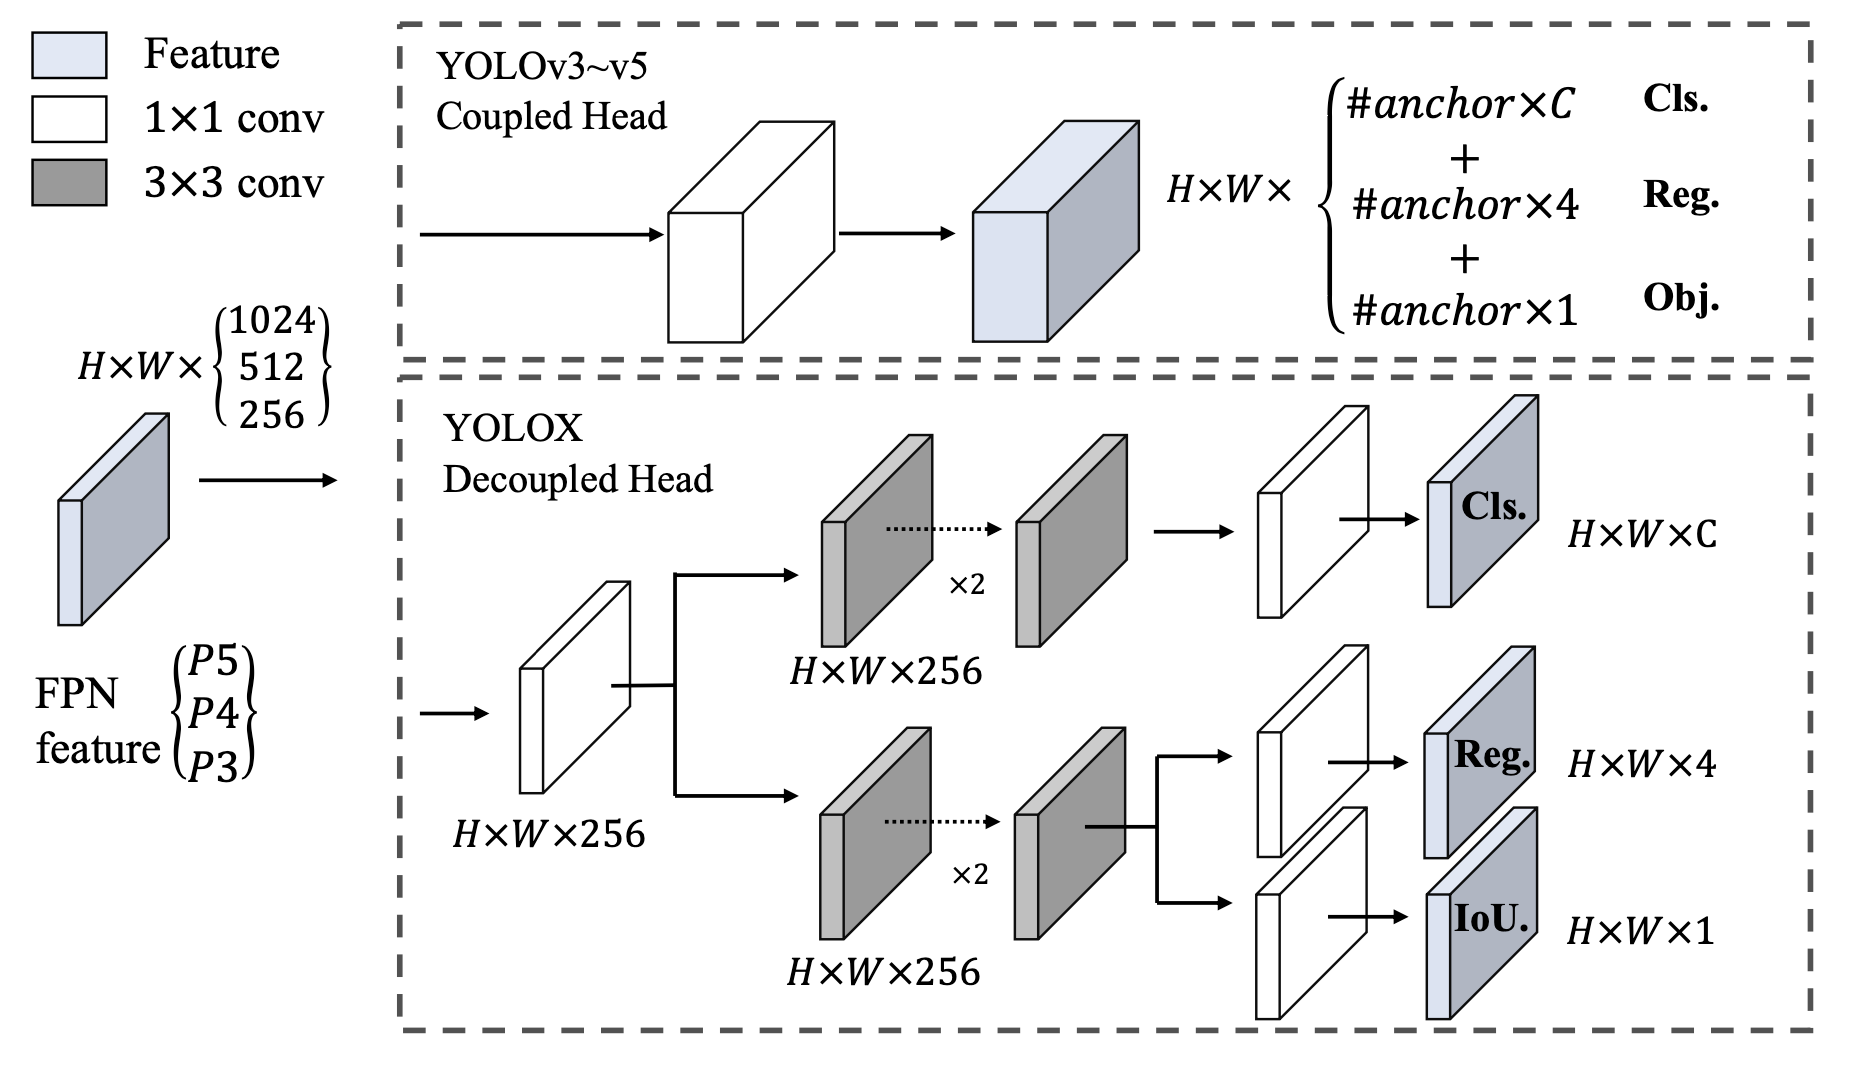
\includegraphics[width=0.55\linewidth]{decoupledHead.png}
	\caption[Illustration des Unterschieds zwischen dem Yolov3-Head und dem neuen Decoupled-Head ]{Illustration des Unterschieds zwischen dem YOLOv3-Head und dem neuen Decoupled-Head Quelle: \cite{yoloxPaper}}
	\label{fig:decoupledHead}
\end{figure}




\subsection{Anchor Free Prediction}\label{chap:anchorFree}
Bei der \textbf{Anchor-based Prediction} werden vordefinierte Ankerboxen verwendet, um Objekte in verschiedenen Größen zu repräsentieren. Diese Ankerboxen dienen als Referenzpunkte, auf die die Modelle während des Trainings ausgerichtet werden. Das Modell weißt der Ground-Truth (Echten) Box die ähnlichste Ankerbox zu und sagt die Verschiebung und Abmessungen der Ankerbox voraus, um sie dem Objekt anzupassen. Dazu muss vor Beginn des Trainings die Skalierung und Anzahl der Ankerboxen vorgegeben werden. Im Grunde ist eine Ankerbox eine Hilfe für das Modell, damit es nicht direkt eine Bounding Box vorhersagen muss.


Die implementierte Methode zur \textbf{Anchor-Free Predictio}n entstammt ursprünglich aus dem Paper ''FCOS: Fully Convolutional One-Stage Object Detection'' \cite{yoloxAnchorFree}. Anstelle von Ankerboxen verwendet die Anchor-Free-Methode ein Grid-basiertes Konzept. Im YOLOX Algorithmus wird eine Stride von 32, 16 und 8 verwendet, um die Ausgabebilder des Necks in ein Gitter zu unterteilen. Wenn ein Stride von 32 für ein 256×256 großes Bild verwendet wird, ergeben sich insgesamt 256/32 = 8 Schnittpunkte in jeder Dimension, also insgesamt 64 Schnittpunkte. Jeder dieser Schnittpunkte heißt Anker-Punkte. Ein Ankerpunkt ist ein Offset, mit dem die (x, y)-Position einer Vorhersage verschoben wird. Die Position des Ankers kann auf dem Bild mit den folgenden Formeln ermittelt werden:
\begin{align}
	x = \frac{s}{2} + s*i, \qquad y = \frac{s}{2} + s*j
\end{align}
Dabei ist s die Schrittweite, i ist der i-te Schnittpunkt auf der x-Achse und j ist der j-te Schnittpunkt auf der y-Achse. Bei YOLOX werden die Gitterpunkte als linker oberer Offset der Bounding Box verwendet. Die folgenden Formeln werden verwendet, um eine vorhergesagte Bounding Box $(p_x, p_y, p_w, p_h)$ auf die tatsächliche Position auf dem Bild $(l_x, l_y, l_w, l_h)$ abzubilden, wenn (x, y) der Schnittpunkt auf dem Gitter ist, zudem die Vorhersage gehört und s die Schrittweite der aktuellen FPN-Ebene ist:
\begin{align}
	l_x=p_x+x, \qquad l_y=p_y+y, \qquad l_w=s*e^{p_w}, \qquad l_h=s*e^{p_h}
\end{align}
Wir verschieben den vorhergesagten Punkt, indem wir die Vorhersage zum Anker-Punkt (dem (x,y)-Punkt, der dieser Vorhersage zugewiesen ist) hinzufügen. Durch die e-Funktion wird sichergestellt, dass die Höhe und Breite nicht negativ ist und verschieben diese auf der Grundlage der Schrittweite s eines Bildes. Das Beispiel zu dieser Methode kann in der angegeben Quelle nachgelesen werden. \cite{yoloxExplanationHowWorks}


\subsection{SimOTA Label Assignment}
Die Methode soll die Zuordnung der Vorhersagen zu den Ground-Truth-Objekten optimieren, da nicht alle Vorhersagen gut sind und das Modell nicht versuchen soll diese zu optimieren. Dazu werden die Anker-Punkte der vorherigen Methode von \ref{chap:anchorFree} in positive und negative Gruppen aufgeteilt. Die positive Gruppe beinhaltet ein Objekt und die negative Gruppe beinhaltet kein Objekt.

OTA (Optimal Transport Assignment) ist ein Ansatz, der das Zuordnungsproblem in der Objekterkennung als Optimal Transport (OT)-Problem formuliert. Es geht darum, den besten Plan zu finden, um Güter (Objekte) von Anbietern (Ground-Truth) zu Nachfragern (Vorhersagen oder Anker) zu minimalen Kosten zu transportieren. OTA verwendet OT, um die Labels den Ankerorten zuzuweisen und die Anker als positiv oder negativ zu kennzeichnen. Der Hintergrund wird als zusätzlicher "Lieferant" betrachtet. 

Das Problem des OTA-Algorithmus ist, dass dieser das Training verlangsamt. Aus diesem Grund gibt es eine Vereinfachung des Algorithmus, indem der optimale Zuweisungsplan angenähert wird. Vereinfacht funktioniert der Algorithmus folgendermaßen:
\begin{itemize}
	\item Berechne die Klassen- und Regressionsvorhersage für eine gegebene Eingabe durch das Modell.
	\item Erstelle einen Liefervektor, der das Angebot (durch Dynamic k estimation festgelegt) für jeden der Ground-Truths repräsentiert.
	\item Initialisiere den Nachfragevektor mit Einsen für jede Vorhersage.
	\item Berechne die Kosten für Klassenverluste ($FocalLoss(P^{cls}, G^{cls})$), Regressionsverluste ($IoULoss(P^{cls}, G^{cls})$))) und Zentrumsprior zwischen Vorhersagen und Ground-Truths.
	\item Berechne die Kosten für den Hintergrund und den Vordergrund basierend auf den Kosten der einzelnen Komponenten.
	\item Konstruiere eine Kostenmatrix, die die Hintergrund- und Vordergrundkosten enthält.
	\item Wähle die besten Vorhersagen basierend auf den Kosten und dem verfügbaren Angebot.
	\item Gebe die ausgewählten Vorhersagen zurück.
\end{itemize}

Der SimOTA-Algorithmus verwendet das Konzept von Angebot und Nachfrage, um die optimale Zuordnung zwischen Vorhersagen und Ground-Truths zu finden. Durch die Berücksichtigung von Kosten und verfügbarem Angebot werden die besten Vorhersagen ausgewählt, um eine präzisere Objekterkennung zu ermöglichen. Der vollständige Algorithmus kann in der angegeben Quelle nachgelesen werden.  \cite{yoloxExplanationSimOTA}


\subsection{Advanced Augmentation}
YOLOX verwendet Advanced Data Augmentation-Techniken wie Mosaic und MixUp, um die Datenvielfalt während des Trainings zu erhöhen und die Leistungsfähigkeit des Modells zu verbessern.

Beim \textbf{Mosaic}-Verfahrenwerden vier zufällig ausgewählte Bilder aus dem Trainingsdatensatz genommen und zu einem Mosaikbild kombiniert. Dabei werden die Bilder in vier quadratische Bereiche aufgeteilt und zu einem einzigen großen Bild zusammengefügt. Die Bounding Boxes der Objekte werden entsprechend angepasst und die Klassenlabels beibehalten. Mithilfe des CutOuts wird ein beliebiger Teil aus dem Bild ausgeschnitten und die Bounding Boxen noch einmal angepasst. Das Mosaikbild wird dann als Eingabe für das Modell verwendet. Der Grund für die Anwendung von Mosaic liegt darin, dass es die Fähigkeit des Modells verbessert, mit komplexen Szenarien und Überlappungen von Objekten umzugehen

\textbf{MixUp} ist eine Technik, bei der zwei zufällig ausgewählte Bilder und ihre entsprechenden Bounding Boxes und Klassenlabel gemischt werden, indem ihre Annotationen gewichtet kombiniert werden. Das erste Bild wird mit $\lambda$ und das zweite Bild mit $1-\lambda$ multipliziert. Die beiden resultierenden Ergebnisse werden addiert. \cite{yoloxExplanationAug}

\begin{figure}[h]
	\centering
	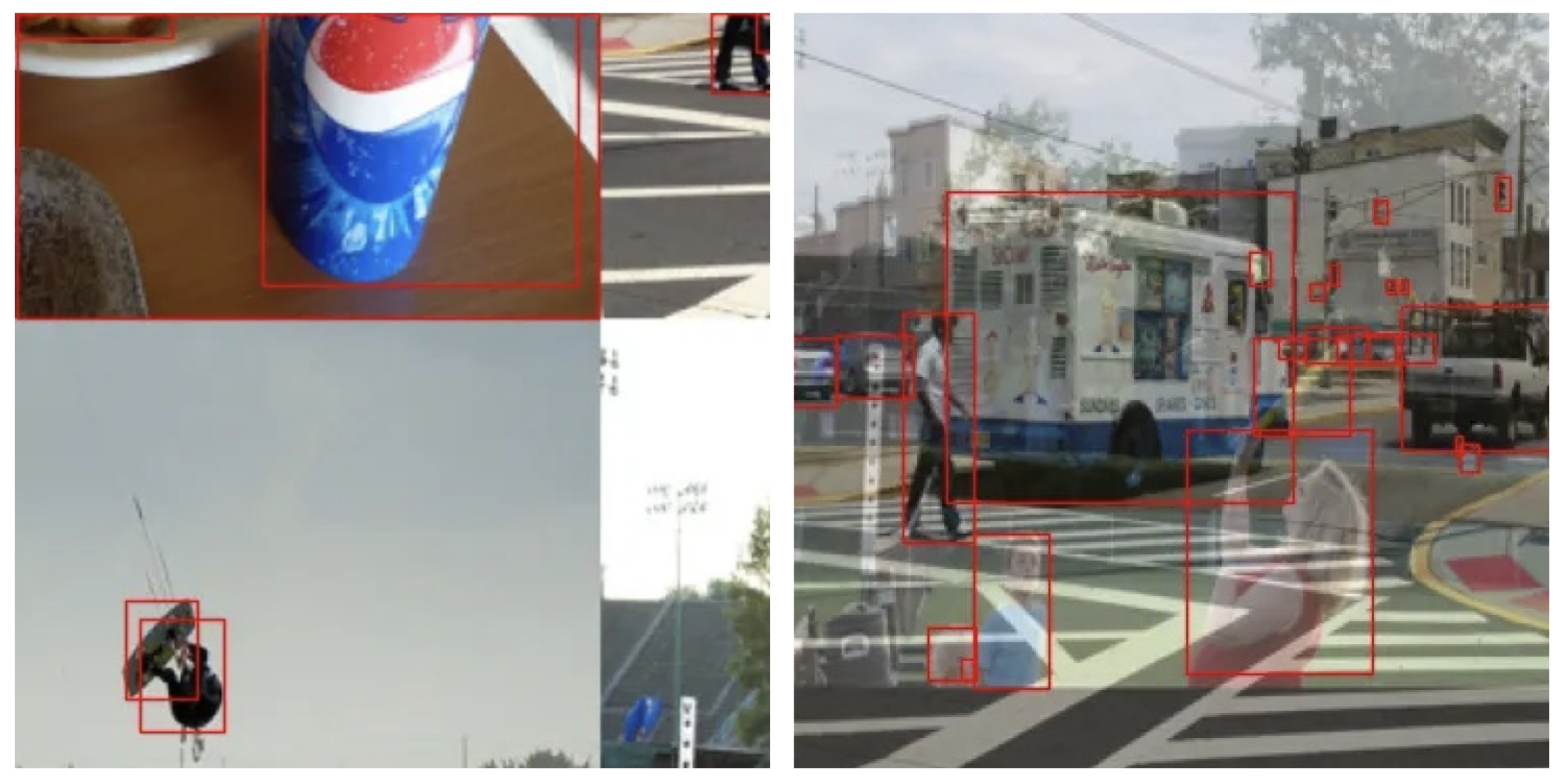
\includegraphics[width=0.55\linewidth]{dataAugmentation.png}
	\caption[Beispielbild nach Anwendung der beiden Data Augmentation Methoden]{Beispielbild nach Anwendung der beiden Data Augmentation Methoden (links: Mosaic, rechts: MixUp) Quelle: \cite{yoloxExplanationAug}}
	\label{fig:yoloxExplanationAug}
\end{figure}



\section{Verlustfunktion}
\subsection{Klassen}
Die Gesamtverlustfunktion des Modells setzt sich aus drei einzelnen Verlustfunktionen für die jeweiligen Aufgaben zusammen:

\begin{align}
	\mathcal{L}^{total}=\frac{1}{N_{pos}}*\mathcal{L}^{cls}+\alpha*\frac{1}{N_{pos}}*	\mathcal{L}^{total}+	\frac{1}{N_{pos}}*\mathcal{L}^{obj}
\end{align}

Die Verlustfunktion ist dabei die Summe der einzelnen Komponenten, gemittelt über die Menge der positiven Labels. Die positiven Labels sind durch SimOTA (\ref{simota}) berechnet. Der Parameter $\alpha$ ist ein Gewichtungsterm, der von den Autoren des Papers auf $5.0$ festgelegt ist.

\subsection{Klassifikation}\label{chap:yoloxClassification}
Für die Verlustfunktion des Klassifikationsteils verwendet YOLOX die Binary Cross Entropy (BCE) mit Logits. Dabei handelt es sich um die normale BCE-Funktion mit einer vorgeschalteten Sigmoidfunktion für die Prognosen.

Die Formel lautet:
\begin{align}
	\mathcal{L}^{cls}=\frac{1}{N}\sum_{i}^{N}y_i*log(\sigma(\hat{y_i}))+(1-y_i)*log(1-\sigma(\hat{y}_i)),
\end{align}

wobei $\hat{y}$ der Vektor der Klassenvorhersagen für C Klassen ist. Die Sigmoidfunktion $\sigma$ wird verwendet, um die Elemente in einem Wertebereich von [0,1] zu abzubilden. Die Werte in y sind ein One-Hot-Vektor, der eine 1 für die richtige Klasse und eine 0 für alle anderen Klassen enthält. Die Werte der Vektoren y und $\hat{y}$ stammen aus der positiv gekennzeichneten Menge. Das Ziel des BCE-Verlustes ist, dass das Modell lernt, eine 1 für die richtige Klasse und eine 0 für alle anderen Klassen in der Bounding Box vorherzusagen. \cite{yoloxExplanationHowWorks}

\subsection{Bounding Box}
In YOLOX wird die IoU (Intersection over Union) Loss Funktion verwendet, um die Regressionsverluste für die Bounding Box Koordinaten zu berechnen. Diese Loss Funktion misst die Ähnlichkeit zwischen der vorhergesagten Bounding Box und der Ground Truth Bounding Box anhand des IoU-Werts.

Der IoU-Wert wird berechnet, indem der Flächenanteil des überlappenden Bereichs der Bounding Boxen durch die Summe der Flächen beider Bounding Boxen geteilt wird. Mathematisch kann der IoU-Wert wie folgt ausgedrückt werden:

\begin{align}
	IoU = \frac{Area_{Intersection}}{Area_{Unoin}}, \qquad IoU \in [0,1]
\end{align}

Je höher der IoU-Wert, desto besser ist die Übereinstimmung zwischen der Vorhersage und der Ground Truth Bounding Box.

Die resultierende Verlustfunktion wird folgendermaßen definiert:
\begin{align}
	\mathcal{L}^{reg} = \frac{1}{N}\sum_{i}^{N}(1-IoU_i)^2,
\end{align}

wobei N die Anzahl der positiven Elemente ist und die Bounding Boxen aus dieser Menge entstammen. \cite{yoloxExplanationHowWorks}

\subsection{Objectness}
Das Ziel des Objectness Loss in YOLOX ist es, dass das Modell einen Wert nahe 1 hat, wenn es glaubt, dass sich ein Objekt in der Bounding Box befindet, einen Wert nahe 0, wenn es glaubt, dass sich nichts in der Box befindet, und einen Wert dazwischen (vorzugsweise etwa 0.5), wenn es unsicher ist.

Um den Wert zu optimieren wird die Binary Cross Entropy with Logits verwendet, die Funktion die auch in \ref{chap:yoloxClassification} verwendet wird. Dabei werden die positiven und negativen Labels von SimOTA verwendet.

Für die positive Vorhersagen wird der IoU-Wert zwischen vorhergesagter und Ground Truth Bounding Box verwendet, um den Wert zu bestimmen, den das Modell vorhersagen soll. Bei negativen Vorhersagen wird der größte IoU-Wert zwischen der vorhergesagten negativen Bounding Box und allen Ground Truth Bounding Boxen verwendet, um die Ground Truth Bounding Box für die negative Vorhersage zu bestimmen. \cite{yoloxExplanationHowWorks}

\section{Modellauswertung}



